\documentclass[aps,superscriptaddress,twocolumn,nopreprintnumbers,floatfix,groupedaddress]{revtex4-1}
\usepackage{amssymb}
\usepackage{amsmath}
\usepackage{graphicx}
\usepackage{dcolumn}
\usepackage{hyperref}
\usepackage{color,units}
\usepackage{lineno}
\usepackage{xspace}
\usepackage{mathtools}
\usepackage{physics}
\usepackage{acronym}
\usepackage{subfigure}
\usepackage{multirow}
\usepackage{tikz}

\newcommand{\bilby}{{\sc Bilby}\xspace}
\newcommand{\lal}{{\sc LAL}\xspace}
\newcommand{\lalsuite}{{\sc LALSuite}\xspace}
\newcommand{\lalsimulation}{{\sc LALSimulation}\xspace}
\newcommand{\sur}{{\sc NRHybSur3dq8}\xspace}
\newcommand{\Z}{\mathcal{Z}}
\newcommand{\M}{\mathcal{M}}
\renewcommand{\L}{\mathcal{L}}
\newcommand{\BF}{\mathcal{BF}}
\newcommand{\proposal}{proposal}
\newcommand{\target}{target}
\newcommand{\ep}[1]{\textcolor{red}{[EP: #1]}}
\newcommand{\et}[1]{\textcolor{blue}{[ET: #1]}}
\newcommand{\ct}[1]{\textcolor{green}{[CT: #1]}}


\newcommand{\emcee}{{\sc emcee}\xspace}
\newcommand{\ptemcee}{{\sc ptemcee}\xspace}
\newcommand{\nessai}{{\sc Nessai}\xspace}
\newcommand{\vitamin}{{\sc VItamin}\xspace}
\newcommand{\bilbypipe}{{\sc bilby\_pipe}\xspace}
\newcommand{\lalinference}{{\sc LALInference}\xspace}
\newcommand{\dynesty}{{\sc dynesty}\xspace}
\newcommand{\cpnest}{{\sc cpnest}\xspace}
\newcommand{\nflows}{{\sc nflows}\xspace}
\newcommand{\pytorch}{{\sc PyTorch}\xspace}
\newcommand{\corner}{{\sc corner}\xspace}
\newcommand{\matplotlib}{{\sc matplotlib}\xspace}
\newcommand{\seaborn}{{\sc seaborn}\xspace}
\newcommand{\numpy}{{\sc NumPy}\xspace}
\newcommand{\scipy}{{\sc SciPy}\xspace}
\newcommand{\pandas}{{\sc pandas}\xspace}
\newcommand{\python}{{\sc Python}\xspace}
\newcommand{\imrphenomp}{{\sc IMRPhenomPv2}\xspace}


\newcommand{\figwidth}{8.6cm}
\newcommand{\onehalffigwidth}{12.9cm}
\newcommand{\doublefigwidth}{17.2cm}
\newcommand{\montefigwidth}{11cm}
\newcommand*{\checktikz}[1][]{\tikz[x=1em, y=1em]\fill[#1] (0,.35) -- (.25,0) -- (1,.7) -- (.25,.15) -- cycle;}


\begin{document}



\title{Explainable Deep-learning: Monte Carlo methods for Gravitational-Wave Inference}

\author{Project No:~628}
\affiliation{%
	SUPA, School of Physics and Astronomy \\
	University of Glasgow \\
	Glasgow G12 8QQ, United Kingdom}%

\date{\today}

\begin{abstract}
My 250 word abstract goes here...
\end{abstract}

\maketitle

\acrodef{GW}[GW]{Gravitational wave}
\acrodef{BBH}[BBH]{binary black hole}
\acrodef{EM}[EM]{electromagnetic}
\acrodef{CBC}[CBC]{compact binary coalescence}
\acrodef{BNS}[BNS]{binary neutron star}
\acrodef{NSBH}[NSBH]{neutron star black hole}
\acrodef{PSD}[PSD]{power spectral density}
\acrodef{ELBO}[ELBO]{evidence lower bound}
\acrodef{LIGO}[LIGO]{advanced Laser Interferometer Gravitational wave Observatory}
\acrodef{CVAE}[CVAE]{conditional variational autoencoder}
\acrodef{KL}[KL]{Kullback--Leibler}
\acrodef{GPU}[GPU]{graphics processing unit}
\acrodef{LVC}[LVC]{LIGO-Virgo Collaboration}
\acrodef{PP}[p-p]{probability-probability}
\acrodef{SNR}[SNR]{signal-to-noise ratio}

\section{Introduction}\label{intro}

Remember to signpost rest of paper at end of this section!

\subsection{Parameter Estimation}

\begin{table}[t]
	\centering
	\caption{}
	\begin{tabular}[t]{lcccc}
		\toprule
		parameter name & symbol & status & value & units\\
		\hline
		mass 1 & $m_1$ & inferred  & 35-80 & \(\textup{M}_\odot\)\\
		mass 2 & $m_2$ & inferred & 35-80 & \(\textup{M}_\odot\)\\
		luminosity distance & $d_{\text{L}}$ & inferred & 1-3 & Gpc\\
		time of coalescence & $t_{0}$ & inferred & 0.65-0.85 & s\\
		inclination & $\Theta_{jn}$ & inferred & 0-$\pi$ & rad\\
		polarisation & $\psi$ & inferred & 0-$\pi$ & rad\\
		\hline
		right ascension & $\alpha$ & fixed & 0 & rad\\
		declination & $\delta$ & fixed & 0 & rad\\
		spins & - & fixed & 0 & -\\
		\hline
		phase at coalescence & $\phi_{0}$ & marginalised & 0-$2\pi$ & rad\\
		\botrule
	\end{tabular}
	\label{tab:prior_ranges}
\end{table}



\begin{align}\label{eq:bayes_exact} 
	p(x|y) = \frac{{\cal L}(y|x) p(x)}{\cal Z} ,
\end{align}

\begin{align}\label{eq:bayes_prop} 
	p(x|y) &\propto {\cal L}(y|x) p(x), 
\end{align}

\begin{align}\label{eq:bayes_evidence} 
{\cal Z} = \int dx {\cal L}(y|x) p(x) ,
\end{align}

Need to know if equation is at end of sentence then swap comma for full stop



\subsection{Deep-learning Approaches}

\subsection{\vitamin: User-friendly Inference}\label{vit}

\begin{align}\label{eq:cross_ent} 
H(p,r) &= -\int dx\, p(x|y) \log r_{\theta}(x|y),
\end{align}

\begin{align}\label{eq:prop_post}
r_{\theta}(x|y) = \int dz\,r_{\theta_1}(z|y)r_{\theta_2}(x|y,z).
\end{align}


Use gen pap to intro CVAE in context, CONTEXT IS KEY HERE


\begin{figure}
	\centering
	
\includegraphics[width=\figwidth]{figs/network_setup.png}
	\caption{}
	\label{fig:vit_flow}
\end{figure}

%
%\subsection{Structure}
%
%\subsection{Training}
%
%\subsection{Results}

%\section{Theoretical Framework}\label{theory}

Need to mention metropolis hastings it seems!

Introduce equations directly to our specifics, we don't have space to intro them blind then again to specifics...

%\subsection{Monte Carlo Framework}\label{theory:monte}

%\subsection{SIR Framework}\label{theory:sir}

Do theory on normal IS and then say that SIR is an monte carlo approach/approx to normal IS then give equations for bot (talk about the NEW IMPROVED SIR method (link to Section \ref{future}))

%
%\subsection{Theoretical Framework}\label{monte:theory}

\section{Methodology}\label{methods}

Apply the intro/theory mateiral to our case, JUSTIFY scientific decisions like number of samples, batch size, npars!!

\subsection{Model Training}

\begin{align}\label{eq:cost_approx} H \lesssim
\frac{1}{N}\sum_{n=1}^{N_{\text{b}}}&\Big[\overbrace{-\log
	r_{\theta_{2}}(x_{n}|z_{n},y_{n})}^{L}\nonumber\\
&+\overbrace{\text{KL}\left[q_{\phi}(z|x_{n},y_{n})||r_{\theta_{1}}(z|y_{n})\right]}^{\text{KL}}\Big],
\end{align}


\begin{figure}
	\centering
	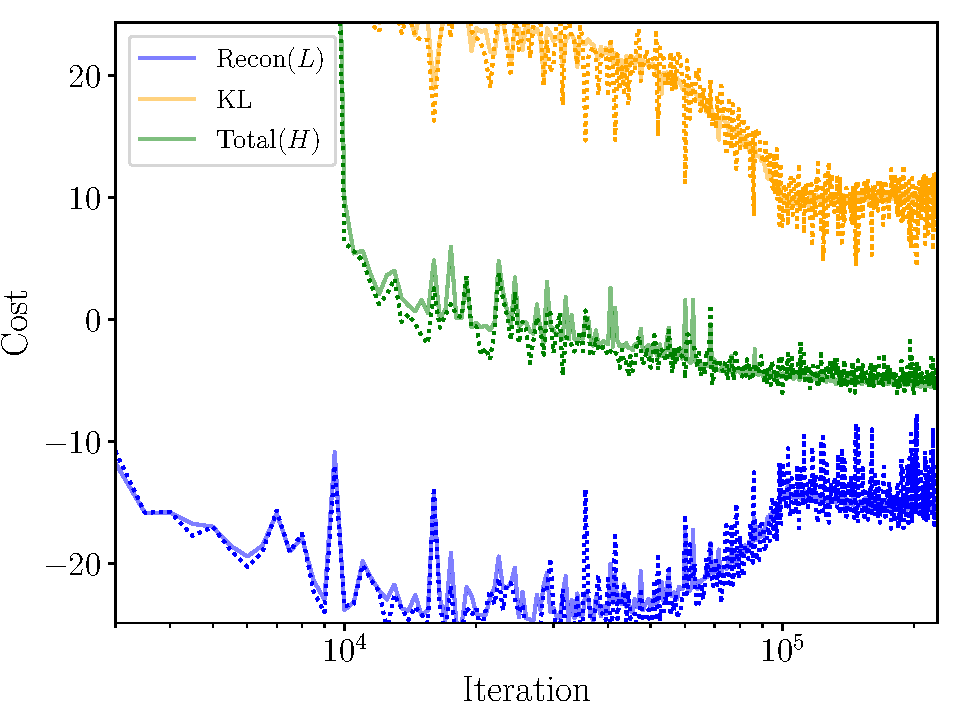
\includegraphics[width=\figwidth]{figs/cost.pdf}
	\caption{}
	\label{fig:learning_contours}
\end{figure}

\begin{figure*}
	\subfigure{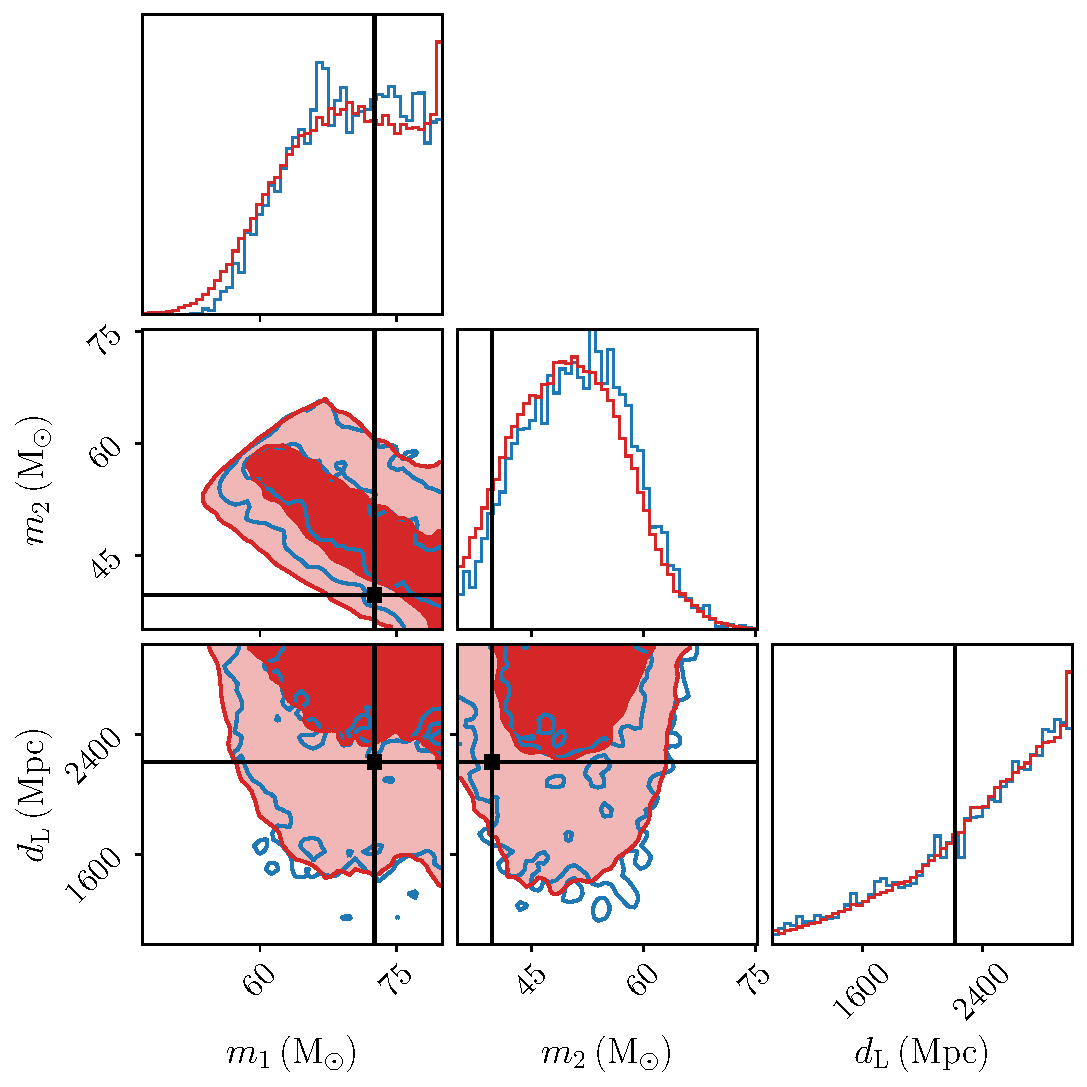
\includegraphics[width=\figwidth]{figs/vit_train_corner1.pdf}}
	\subfigure{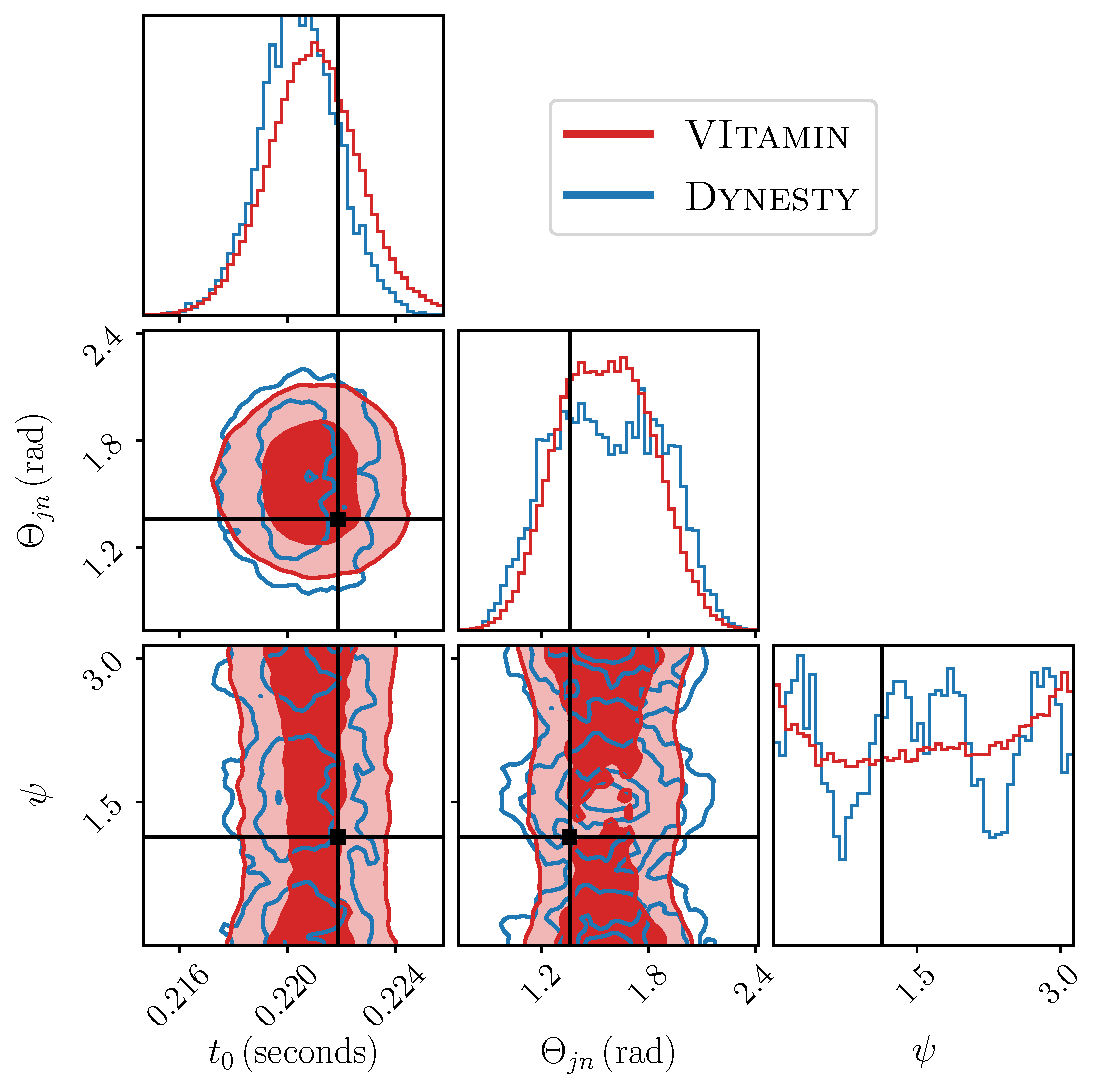
\includegraphics[width=\figwidth]{figs/vit_train_corner2.pdf}}
	\caption{Probability-probability (P-P) plot showing the confidence interval versus the fraction of the events within that confidence interval for the posterior distributions obtained using our analysis \nessai for 128 simulated compact binary coalescence signals produced with \bilby and \bilbypipe. The 1-, 2- and 3-$\sigma$ confidence intervals are indicated by the shaded regions and $p$-values are shown for each of the parameters and the combined $p$-value is also shown.}
	\label{fig:vit_train_corner}
\end{figure*}


\subsection{Likelihood Estimates}

\begin{align}\label{eq:monte_approx}
	r_{\theta}(x|y) = & \,\mathbb{E}_{r_{\theta_1}(z|y)}r_{\theta_2}(x|y,z)\nonumber \\
	 \approx & \frac{1}{N}\sum^{N}_{j=1}\left.r_{\theta_{2,j}}(x_i|y,z_j)\right|_{z_j\sim r_{\theta_1}(z_j|y)},
\end{align}

\begin{align}\label{eq:post_like}
r_{\theta}(x|y) \sim {\cal L}_{\theta}(y|x),
\end{align}

\textbf{\textcolor{red}{Figs: Monte flowchart}}

\begin{figure*}
	\centering
	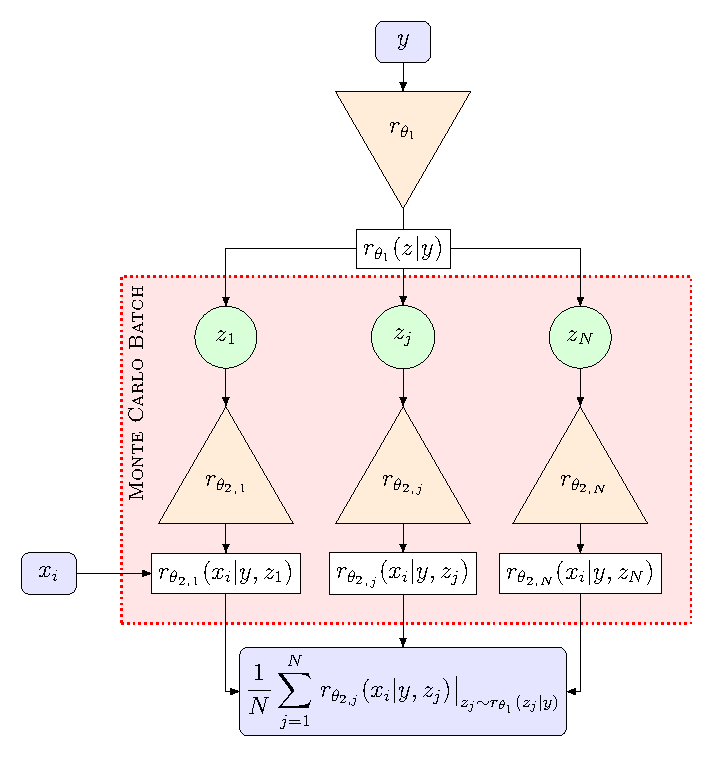
\includegraphics[width=\montefigwidth]{figs/tikz_monte.pdf}
	\caption{}
	\label{fig:monte_flow}
\end{figure*}


\subsection{Likelihood Reweighting}

Start with eq 2 then multiply by unity

\begin{align}\label{eq:sir} 
p(x|y) &\propto \frac{{\cal L}_\theta(y|x)}{{\cal L}_\theta(y|x)}{\cal L}(y|x) p(x)\nonumber\\
&\propto w(y|x)\overbrace{{\cal L}_{\theta}(y|x) p(x)}^{r_{\theta}(x|y)}.
\end{align}

%\begin{table}
%	\centering
%	\caption{Med time to gen 10,000 samples...the DL doesnt account for training time}
%	\begin{tabular}[t]{llcc} 
%				\toprule
%				sampler & method & deep-learning & run-time (s)\\
%				\hline
%				h &&&\\
%				h &&&\\
%%				\emcee~\cite{mcmc_og} & help & help & help\\
%%				help & & &\\
%%				\emcee~\cite{mcmc_og} & help & help & help\\
%%				\emcee~\cite{emcee} & MCMC~\cite{mcmc_og} & X  &  32070\\
%%				\ptemcee~\cite{ptemcee} & MCMC & X & 24372\\
%%				\dynesty~\cite{dynesty} & NS~\cite{skilling2006} & X & 19400\\
%%				\cpnest~\cite{cpnest} & NS & X &  26202 \\
%%				\hline
%%				\nessai~\cite{williams2021nested} & NS & Y & 9372\\
%%				\vitamin~\cite{vitpaper} & VI~\cite{1904.06264} & Y & $1\times 10^{-1}$\\
%				\botrule
%	\end{tabular}
%	\label{Tab:speed}
%\end{table}
Here,

\begin{align}\label{eq:weights}
w(y|x) \equiv \frac{{\cal L}(y|x)}{{\cal L}_{\theta}(y|x)},
\end{align}

is the weight function...

\section{Results}\label{results}

\subsection{Self-consistency}

\begin{figure*}
	\subfigure{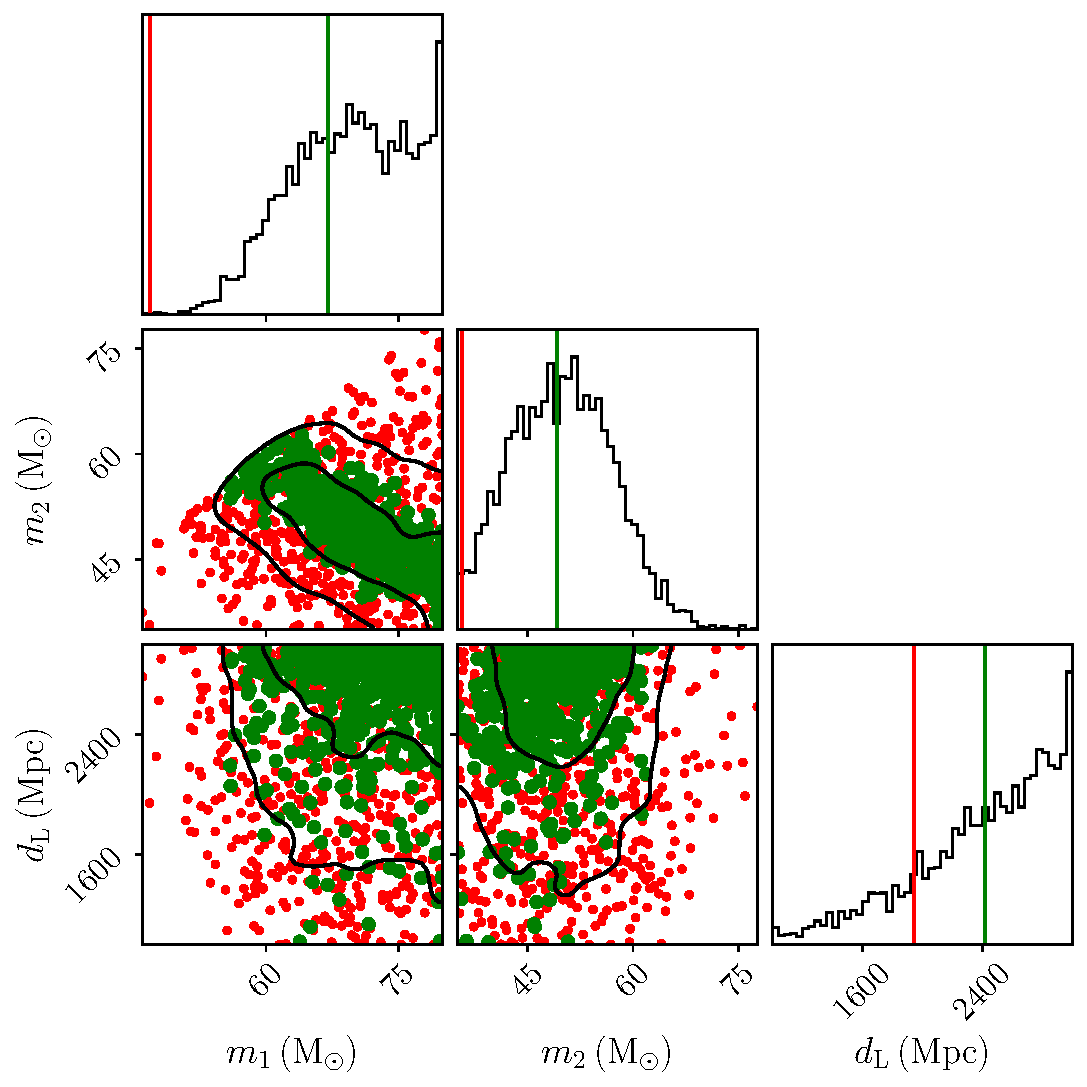
\includegraphics[width=\figwidth]{figs/self_consist1.pdf}}
	\subfigure{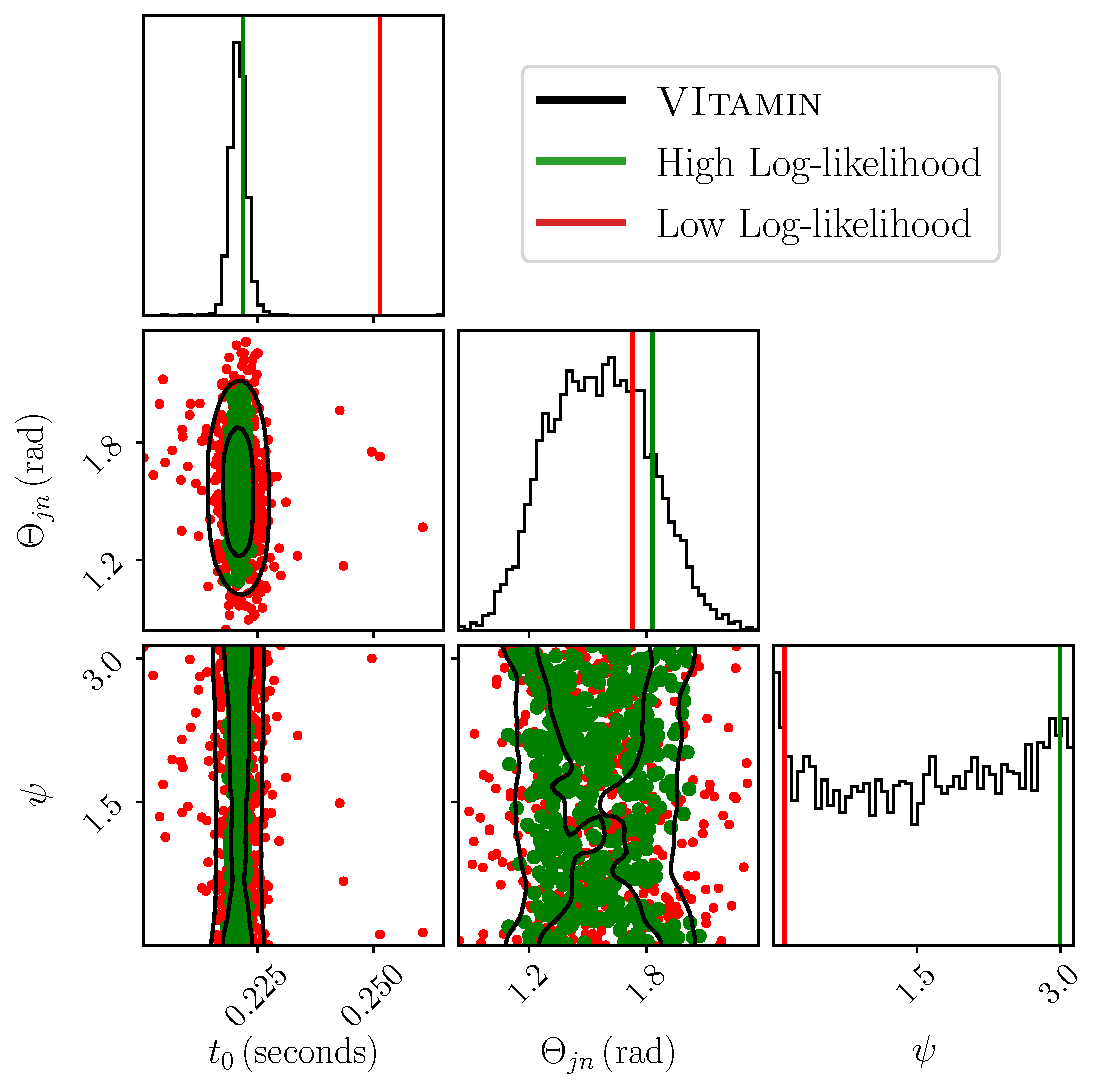
\includegraphics[width=\figwidth]{figs/self_consist2.pdf}}
	\caption{Probability-probability (P-P) plot showing the confidence interval versus the fraction of the events within that confidence interval for the posterior distributions obtained using our analysis \nessai for 128 simulated compact binary coalescence signals produced with \bilby and \bilbypipe. The 1-, 2- and 3-$\sigma$ confidence intervals are indicated by the shaded regions and $p$-values are shown for each of the parameters and the combined $p$-value is also shown.}
	\label{fig:sel_consist}
\end{figure*}


\subsection{Reproducibility}

\begin{align}\label{eq:sigma}
\sigma \propto \frac{1}{\sqrt{N}},
\end{align}

where N is monte carlo batch size

\begin{align}\label{eq:error}
\text{Error} = \frac{\sigma}{\sqrt{n_{\text{samples}}}},
\end{align}



\begin{figure}
	\centering
	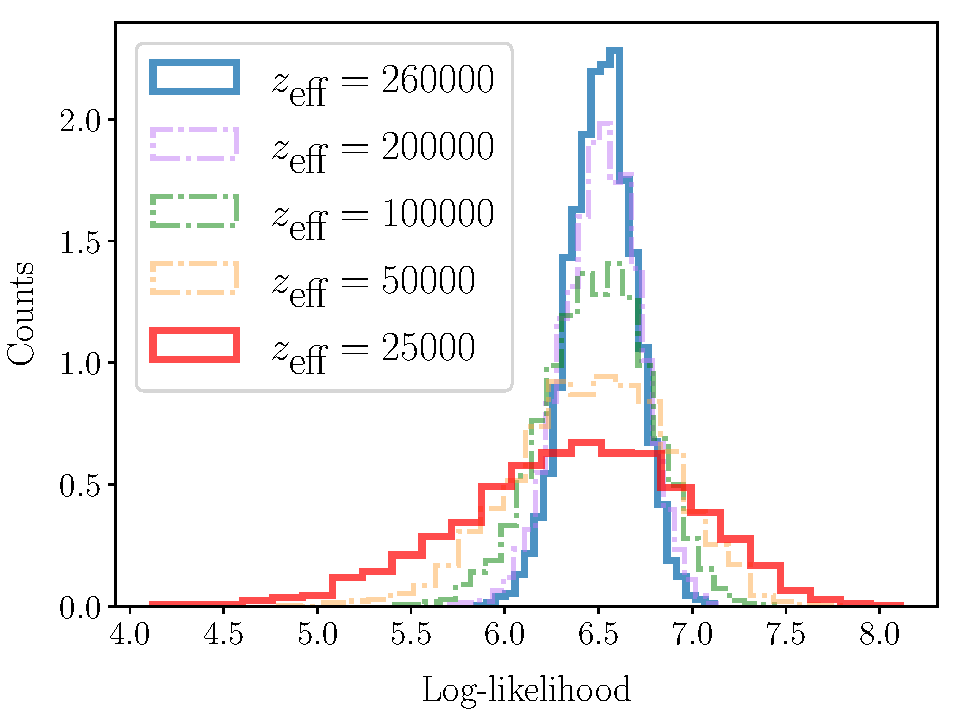
\includegraphics[width=\figwidth]{figs/hists_rect.pdf}
	\caption{}
	\label{fig:hists}
\end{figure}

\begin{figure*}
	\subfigure[]{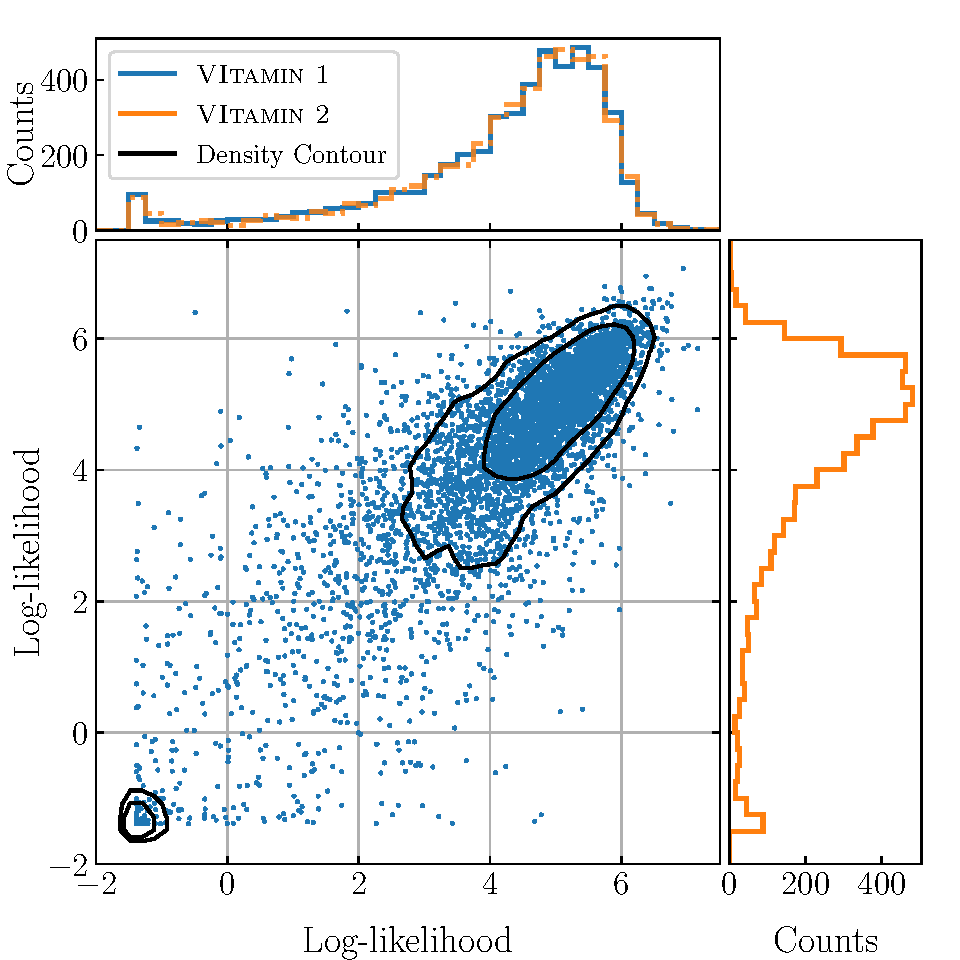
\includegraphics[width=\figwidth]{figs/vvscatter.pdf}}
	\subfigure[]{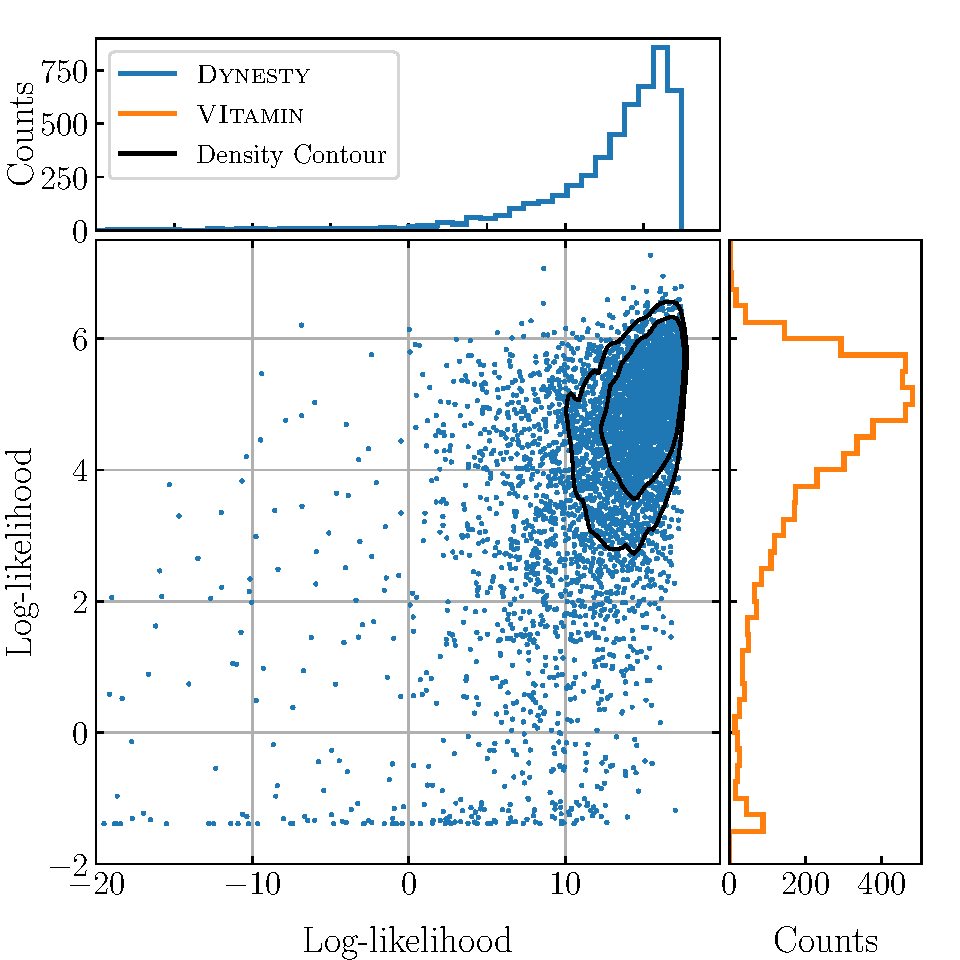
\includegraphics[width=\figwidth]{figs/bvscatter.pdf}}
	\caption{Probability-probability (P-P) plot showing the confidence interval versus the fraction of the events within that confidence interval for the posterior distributions obtained using our analysis \nessai for 128 simulated compact binary coalescence signals produced with \bilby and \bilbypipe. The 1-, 2- and 3-$\sigma$ confidence intervals are indicated by the shaded regions and $p$-values are shown for each of the parameters and the combined $p$-value is also shown.}
	\label{fig:scatter}
\end{figure*}

\subsection{Importance Resampling}


\begin{figure*}[h]
	\centering
	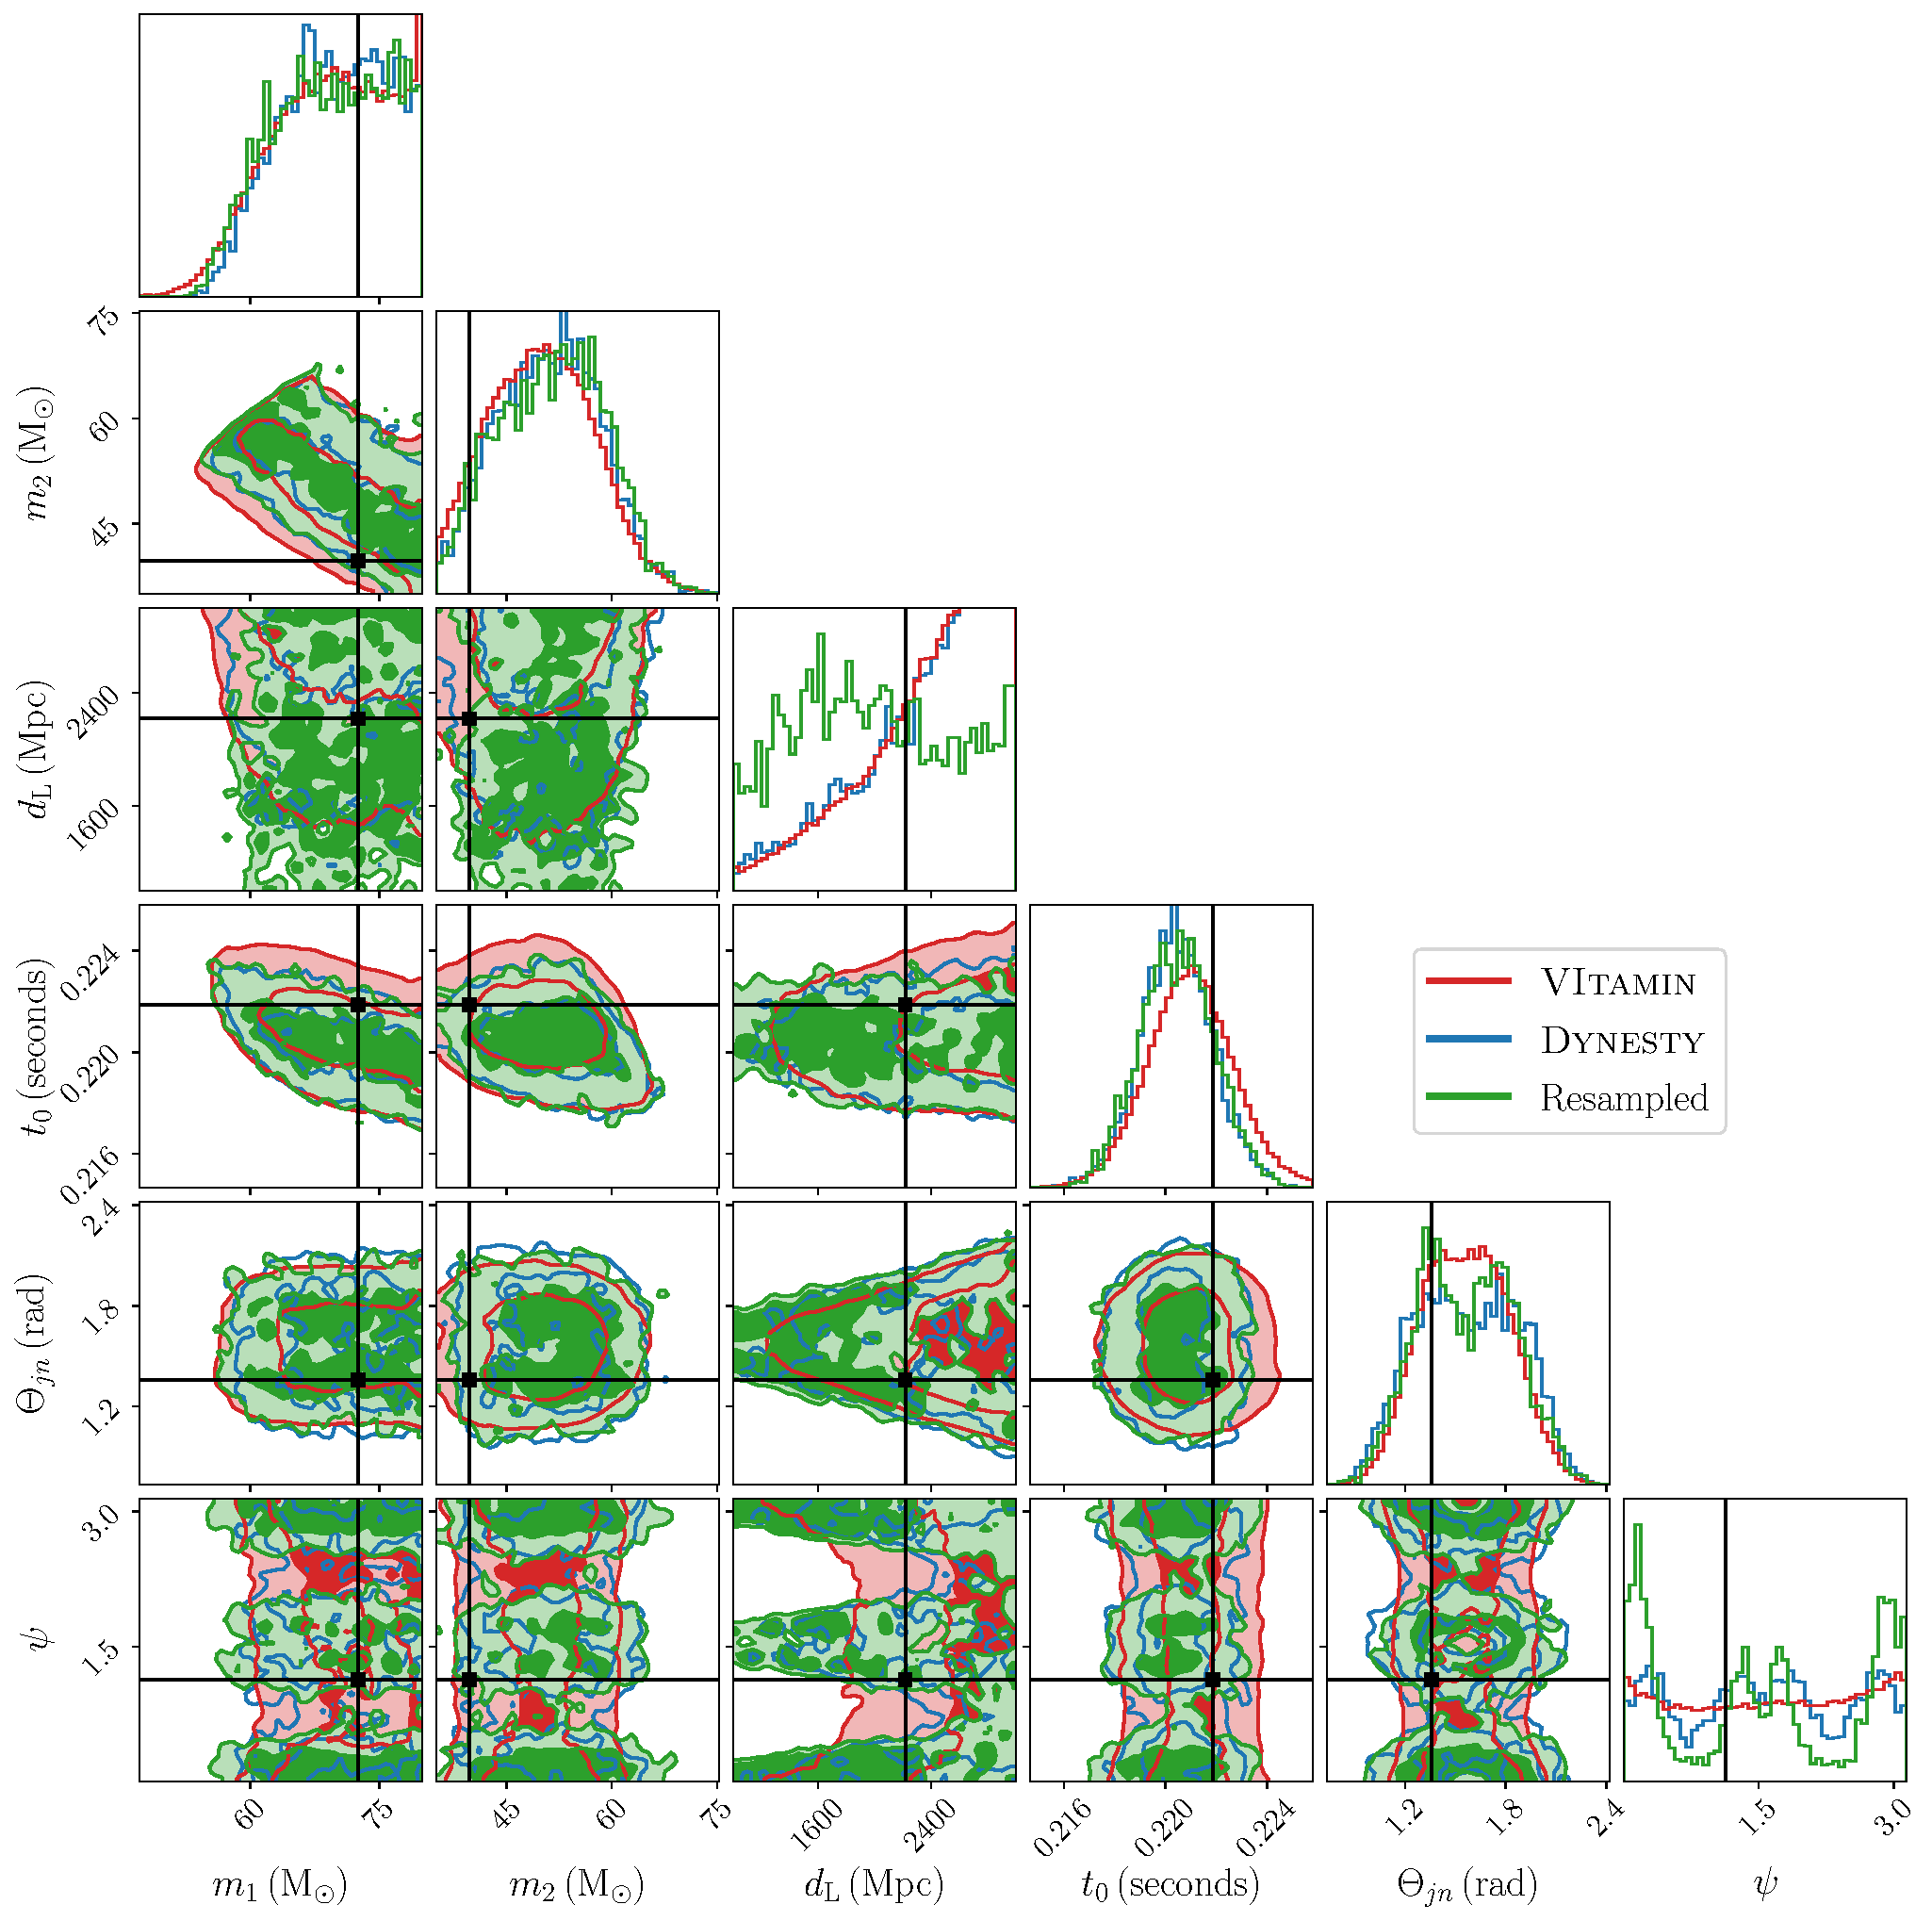
\includegraphics[width=\doublefigwidth]{figs/resample_corner.pdf}
	\caption{}
	\label{fig:final_corner}
\end{figure*}

%\section{Future Work}\label{future}


\section{Conclusions}\label{conc}

This is section has to encapsulate everything we did so that after the abstract a reader can go here and see if they want to buy the paper or not!

As we find ourself in a proof-of-concept mode, there is justification of a section dedicated to the next steps leading towards production of this code.


\section*{Acknowledgements}

Thanks to Chris and Hunter and Michael and Daniel.

Paragraph on the software used \bilby\cite{bilby} \cite{0004-637X-748-2-136}help please dont fuck up now , lets just keep typing and see what happens, im really shitting ymself now... and dont want to have to spend precious time on fucking type setting and bibliography hunting \cite{emcee}
%\clearpage

\begin{table}[t]
	\centering
	\caption{Generic Caption like in vitamin paper!}
	\begin{tabular}[t]{llcc} 
				\toprule
				sampler & algorithm & deep-learning & run-time (s)\footnote{The benchmark samplers all produced $\mathcal{O}(10000)$ samples dependent on the default sampling parameters used, run-time for depp-learning algorihms does not include trainign time}\\
				\hline
				\emcee~\cite{emcee} & MCMC~\cite{mcmc_og} & X  &  32070\\
				\ptemcee~\cite{ptemcee} & MCMC & X & 24372\\
				\dynesty~\cite{dynesty} & NS~\cite{skilling2006} & X & 19400\\
				\cpnest~\cite{cpnest} & NS & X &  26202 \\
				\hline
				\nessai~\cite{williams2021nested} & NS & \checktikz & 9372\\
				\vitamin~\cite{vitpaper} & VI~\cite{1904.06264} & \checktikz & $1\times 10^{-1}$\\
				\botrule
	\end{tabular}
	\label{Tab:speed}
\end{table}

\bibliography{refs}




\end{document}